\section{Results\label{sec:results}}
This section reports the results for code-to-architecture mapping across ten subject systems. RQ1 compares lexical, structural, and contextual file representations using an MLP. RQ2 examines how mapping performance changes when Word2Vec, Node2Vec, and \ft{} initialize HGT with file, member, and folder context, and analyzes errors relative to directory-based predictions. RQ3 uses controlled experiments to examine how using dependency neighbors changes mapping performance, and how the predictor and aggregation direction affect this change.

For RQ1 and RQ2, we report median macro- and micro-F1 scores over the 100 runs per system and configuration, and differences between these medians in F1 percentage points, with Cliff's $\delta$ alongside the significance test. For RQ3, we report the median of the paired differences between conditions over the 100 splits. Summary tables give the median of these per-system values across the ten systems. F1 is computed only on the held-out test files of each split.
% ========================================
% ----------------- RQ1 ------------------
% ========================================
\subsection{Comparing Lexical, Structural, and Contextual File Representations (RQ1)\label{sec:rq1}}

RQ1 examines how much predictive information each file representation provides before additional graph-based message passing. Table~\ref{tab:rq1_mlp_features} reports the median macro-F1 and micro-F1 scores obtained with Word2Vec, Node2Vec, and UniXcoder variants: \zs{} and \ft{}. Each representation is evaluated using the MLP.  
% The classifier performs no message passing, although Node2Vec encodes dependency topology directly and \ft{} incorporates dependency information through its fine-tuning procedure. 

% _________ Results table __________
\begin{table}[ht]
\centering
\small
\renewcommand{\arraystretch}{1.05}
\caption{Median macro-F1/micro-F1 scores (\%) across 100 runs for the feature-only MLP using W2V, N2V, and contextual representation variants: \zs{} and \ft{}. Highlighted values indicate the highest score for each system and metric.\label{tab:rq1_mlp_features}}
\begin{adjustbox}{width=\columnwidth}
\setlength{\tabcolsep}{11pt}
\begin{tabular}{lcccc}
\toprule
System & W2V & N2V & \zs{} & \ft{} \\
\midrule
A.UML
& 34\,/\,57
& \best{54}\,/\,\best{72}
& 36\,/\,60
& 46\,/\,69 \\

C.Img
& 23\,/\,39
& \best{71}\,/\,\best{80}
& 33\,/\,52
& 42\,/\,62 \\

JabRef
& \best{44}\,/\,78
& 40\,/\,74
& 39\,/\,76
& 43\,/\,\best{79} \\

Lucene
& 57\,/\,71
& \best{66}\,/\,\best{79}
& 54\,/\,66
& 63\,/\,76 \\

SH-3D
& 22\,/\,41
& 43\,/\,58
& \best{48}\,/\,64
& 47\,/\,\best{67} \\

T.Mates
& 30\,/\,55
& 41\,/\,68
& 37\,/\,68
& \best{51}\,/\,\best{79} \\

Bash
& 7\,/\,29
& \best{42}\,/\,\best{61}
& 23\,/\,42
& 27\,/\,49 \\

HDF
& 8\,/\,22
& \best{53}\,/\,\best{57}
& 42\,/\,44
& 46\,/\,48 \\

Chrome
& 14\,/\,48
& \best{41}\,/\,\best{71}
& 14\,/\,48
& 31\,/\,66 \\

HDC
& 33\,/\,53
& 43\,/\,69
& 30\,/\,51
& \best{46}\,/\,\best{70} \\

\bottomrule
\end{tabular}
\end{adjustbox}
\end{table}

Macro-F1 is lower than micro-F1 for every system and representation. Node2Vec achieves the highest median macro- and micro-F1 scores on six systems. On the other four systems, \ft{} obtains the highest median micro-F1, while the highest median macro-F1 is held by \ft{} on T.Mates and HDC, Word2Vec on JabRef, and \zs{} on SH-3D.

\parg{Statistical significance of observed differences.} Table~\ref {tab:rq1_stats} summarizes the pairwise differences across all ten systems, with the number of systems favoring each method and the number of Holm-significant differences in each direction.
% _________ Stats table __________
\begin{table}[t]
\centering
\small
\caption{Summary of pairwise differences in F1 points across ten systems. $\Delta$ is the median over systems of the difference between the two configuration medians (first method minus second); $+$ve counts systems favoring the first method; $\uparrow/\downarrow$ gives the number of significant positive/negative differences (paired Wilcoxon, Holm).\label{tab:rq1_stats}}
\begin{adjustbox}{max width=\linewidth}
\begin{tabular}{lrrrrrr}
\toprule
& \multicolumn{3}{c}{Macro F1} & \multicolumn{3}{c}{Micro F1} \\
\cmidrule(lr){2-4}\cmidrule(lr){5-7}
Comparison & $\Delta$ & $+$ve & $\uparrow/\downarrow$ & $\Delta$ & $+$ve & $\uparrow/\downarrow$ \\
\midrule
\zs{}$-$W2V & +4.8 & 6 & 6/4 & +8.0 & 7 & 6/3 \\
\ft{}$-$\zs{} & +9.1 & 9 & 9/0 & +9.5 & 10 & 10/0 \\
\ft{}$-$W2V & +18.0 & 9 & 9/0 & +19.1 & 10 & 9/0 \\
\ft{}$-$N2V & \best{$-$5.2} & 4 & 4/6 & \best{$-$2.9} & 4 & 3/6 \\
N2V$-$W2V & +20.7 & 9 & 9/1 & +16.1 & 9 & 9/1 \\
\bottomrule
\end{tabular}
\end{adjustbox}
\end{table}


We first compare Word2Vec and \zs{}, the two representations that do not encode dependencies. They do not separate consistently: the significant differences fall in both directions, although \zs{} is favored on more systems. On macro-F1, \zs{} is significantly stronger on A.UML (medium effect), C.Img, SH-3D, T.Mates, Bash, and HDF (large effects), whereas Word2Vec is significantly stronger on JabRef (large effect), Lucene and Chrome (medium effects), and HDC (small effect). On micro-F1, \zs{} is significantly stronger on the same six systems, and Word2Vec is significantly stronger on JabRef and Lucene (large effects) and HDC (small effect); the difference in Chrome is not significant.
 
Fine-tuning significantly improves UniXcoder over \zs{} on micro-F1 for all ten systems and on macro-F1 for nine, predominantly with large effects. The effects are medium on HDF (both metrics) and on SH-3D micro-F1; the macro-F1 difference on SH-3D is not significant.

Both representations encoding dependency information are generally stronger than the lexical representation. Node2Vec significantly outperforms Word2Vec on both metrics for nine systems, with JabRef as the exception, where Word2Vec is significantly stronger. Similarly, \ft{} significantly outperforms Word2Vec on both metrics for nine systems; on JabRef, the difference is not significant on either metric.
 
Node2Vec is significantly stronger than \ft{} on both metrics for A.UML, C.Img, Lucene, Bash, HDF, and Chrome, whereas \ft{} is significantly stronger on JabRef, SH-3D, and T.Mates; most of these differences have large effects. On HDC, \ft{} is significantly stronger on macro-F1 with a small effect, and the micro-F1 difference is not significant.

% \FloatBarrier
\begin{GrayBox}{Answer to RQ1.}
Representations that encode dependencies, either directly through random walks (Node2Vec) or through dependency-guided fine-tuning of UniXcoder, provide the strongest mapping performance overall. Fine-tuning consistently improves UniXcoder over its zero-shot representation and produces the best macro-F1 on two systems. Word2Vec and \zs{}, which do not encode dependencies, differ from each other in both directions, and Word2Vec is weaker than Node2Vec and \ft{} on most systems; Word2Vec nevertheless remains stronger than Node2Vec on JabRef. Thus, no single file representation performs best across all systems and metrics.
\end{GrayBox}
% ========================================
% ----------------- RQ2 ------------------
% ========================================
\subsection{Message Passing over Dependency Edges and through Member and Folder Nodes (RQ2) \label{sec:rq2}}

RQ2 examines how mapping performance changes for each representation when message passing over the file dependency graph is added and the graph is extended with folder and member nodes. Figure~\ref{fig:rq2_lineplot} reports median macro-F1 and micro-F1 for the MLP and HGT under F, FF, FM, and FFM. We use Word2Vec, Node2Vec, and the fine-tuned variant \ft{}, which improves over \zs{} on nearly all systems (RQ1). F adds message passing over file dependencies, FF adds folder nodes, FM adds member nodes, and FFM adds both.

Table~\ref{tab:rq2_steps} summarizes five steps: MLP to F, adding members (F to FM, FF to FFM), and adding folders (F to FF, FM to FFM). For each system, $\Delta$ is the difference between the two configuration medians over 100 runs. The table reports the median of these ten system-level differences, the number of systems with a positive difference, and the number of systems with a significant gain or loss.
%_______________
\begin{figure*}[htb]
\centering
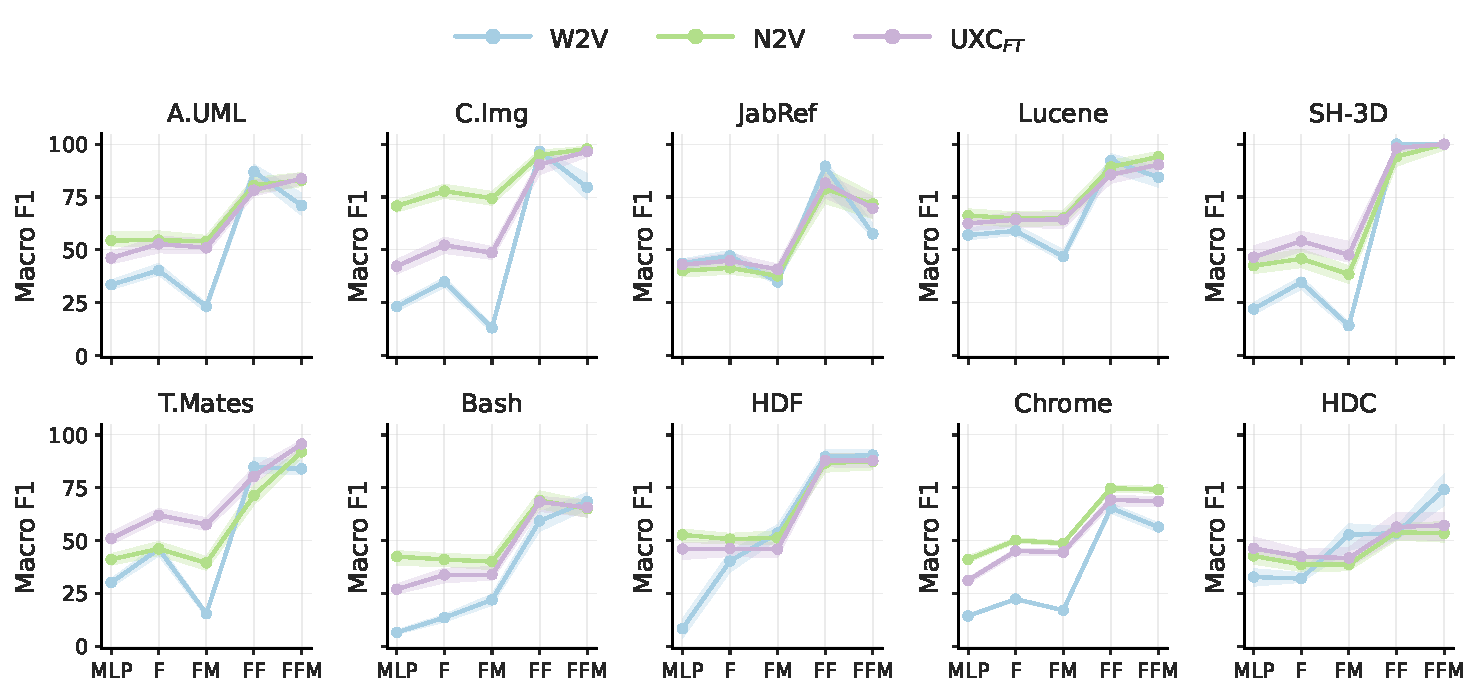
\includegraphics[width=1\textwidth]{Images/RQ2_lineplot_f1_macro.pdf}
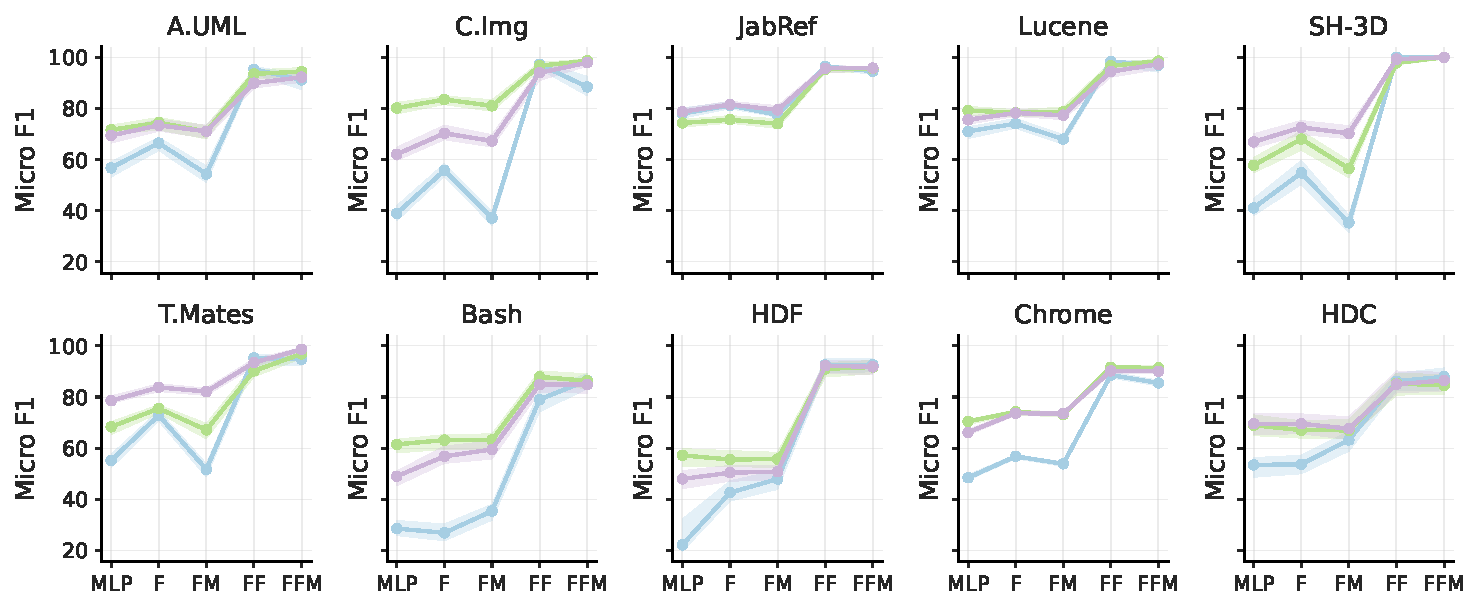
\includegraphics[width=1\textwidth]{Images/RQ2_lineplot_f1_micro.pdf}
\caption{Median macro-F1 (top) and micro-F1 (bottom) for each representation, per system, across the MLP and HGT with increasing graph structure (F, FF, FM, FFM). Shaded areas denote interquartile ranges across the 100 runs. \label{fig:rq2_lineplot}}
\end{figure*}
\begin{table*}[t]
\centering
\caption{Change in macro- and micro-F1 as graph structure is added, by representation. Each row compares the later configuration with the earlier one. Each cell gives the median difference across ten systems in F1 points, followed in parentheses by the number of systems with a positive difference and the numbers of significant positive and negative differences. Shading marks the median difference: blue for gains, purple for losses, and darker for larger changes.\label{tab:rq2_steps}}
\begin{adjustbox}{max width=\textwidth}
\setlength{\tabcolsep}{12pt}
\renewcommand{\arraystretch}{1.2}
\begin{tabular}{lrrrrrr}
\toprule
& \multicolumn{2}{c}{W2V} & \multicolumn{2}{c}{N2V} & \multicolumn{2}{c}{\ft{}} \\
\cmidrule(lr){2-3}\cmidrule(lr){4-5}\cmidrule(lr){6-7}
Step & Macro F1 & Micro F1 & Macro F1 & Micro F1 & Macro F1 & Micro F1 \\
\midrule
F $-$ MLP & \gc{45}+1.6 (6; 6/3) & \gc{45}+1.2 (6; 6/2) & \rc{45}$-$2.9 (1; 1/5) & \rc{70}$-$3.2 (2; 2/6) & \gc{45}+2.9 (8; 4/1) & \gc{25}+0.9 (7; 3/1) \\
FM $-$ F & \gc{45}+1.5 (6; 5/3) & \gc{45}+2.6 (7; 6/3) & \gc{25}+0.9 (6; 4/0) & \gc{45}+2.3 (7; 6/2) & \gc{45}+1.5 (7; 2/2) & \gc{45}+1.8 (8; 6/2) \\
FFM $-$ FF & \gc{100}+11.2 (10; 10/0) & \gc{70}+4.5 (10; 9/0) & \gc{70}+3.3 (8; 5/1) & \gc{45}+2.5 (8; 5/0) & \gc{70}+4.4 (8; 7/0) & \gc{45}+2.5 (10; 6/0) \\
FF $-$ F & \gc{100}+32.9 (10; 10/0) & \gc{100}+33.7 (10; 10/0) & \gc{100}+18.1 (10; 10/0) & \gc{100}+16.7 (10; 10/0) & \gc{100}+27.9 (10; 10/0) & \gc{100}+19.8 (10; 10/0) \\
FFM $-$ FM & \gc{100}+47.2 (10; 10/0) & \gc{100}+37.6 (10; 10/0) & \gc{100}+17.4 (10; 10/0) & \gc{100}+16.9 (10; 10/0) & \gc{100}+36.5 (10; 10/0) & \gc{100}+22.2 (10; 10/0) \\
\bottomrule
\end{tabular}
\end{adjustbox}
\end{table*}

% \begin{table*}[t]
% \centering
% \caption{Changes in Macro and F1 as graph structure is added, by representation. Rows compare the later configuration with the earlier one. $\Delta$ is the median difference across nine systems; $+$ve counts positive differences; $\uparrow/\downarrow$ gives the numbers of significant positive and negative differences, respectively (Wilcoxon signed-rank test, Holm-adjusted, $\alpha=0.05$). Shading marks $\Delta$: blue for gains, purple for losses, darker for larger changes.\label{tab:rq2_steps}}
% \begin{adjustbox}{max width=\textwidth}
% \large
% \begin{tabular}{lrrrrrrrrrrrrrrrrrrr}
% \toprule
% & \multicolumn{6}{c}{W2V} & \multicolumn{6}{c}{N2V} & \multicolumn{6}{c}{\ft{}} \\
% \cmidrule(lr){2-7}\cmidrule(lr){8-13}\cmidrule(lr){14-19}
% & \multicolumn{3}{c}{Macro F1} & \multicolumn{3}{c}{Micro F1}
% & \multicolumn{3}{c}{Macro F1} & \multicolumn{3}{c}{Micro F1}
% & \multicolumn{3}{c}{Macro F1} & \multicolumn{3}{c}{Micro F1} \\
% \cmidrule(lr){2-4}\cmidrule(lr){5-7}
% \cmidrule(lr){8-10}\cmidrule(lr){11-13}
% \cmidrule(lr){14-16}\cmidrule(lr){17-19}
% Step
% & $\Delta$ & $+$ve & $\uparrow/\downarrow$
% & $\Delta$ & $+$ve & $\uparrow/\downarrow$
% & $\Delta$ & $+$ve & $\uparrow/\downarrow$
% & $\Delta$ & $+$ve & $\uparrow/\downarrow$
% & $\Delta$ & $+$ve & $\uparrow/\downarrow$
% & $\Delta$ & $+$ve & $\uparrow/\downarrow$ \\
% \midrule
% F $-$ MLP
% & \gc{45}+1.8 & 6 & 6/2 & \gc{45}+1.5 & 6 & 6/3
% & \rc{45}$-$2.7 & 1 & 1/5 & \rc{45}$-$2.1 & 2 & 2/5
% & \gc{70}+3.7 & 7 & 6/1 & \gc{45}+1.2 & 7 & 7/1 \\
% FM $-$ F
% & \gc{25}+0.5 & 5 & 5/4 & \gc{45}+2.7 & 6 & 6/3
% & \gc{25}+0.1 & 5 & 3/1 & \gc{45}+1.5 & 6 & 6/3
% & \gc{45}+1.5 & 6 & 6/2 & \gc{45}+1.6 & 7 & 7/2 \\
% FFM $-$ FF
% & \gc{100}+10.1 & 9 & 9/0 & \gc{70}+4.0 & 9 & 9/0
% & \gc{45}+1.9 & 7 & 4/1 & \gc{45}+2.0 & 7 & 5/1
% & \gc{70}+3.6 & 7 & 7/0 & \gc{45}+2.4 & 9 & 9/0 \\
% FF $-$ F
% & \gc{100}+29.9 & 9 & 9/0 & \gc{100}+38.7 & 9 & 9/0
% & \gc{100}+19.0 & 9 & 9/0 & \gc{100}+16.4 & 9 & 9/0
% & \gc{100}+27.7 & 9 & 9/0 & \gc{100}+20.6 & 9 & 9/0 \\
% FFM $-$ FM
% & \gc{100}+45.5 & 9 & 9/0 & \gc{100}+38.8 & 9 & 9/0
% & \gc{100}+18.5 & 9 & 9/0 & \gc{100}+18.7 & 9 & 9/0
% & \gc{100}+35.9 & 9 & 9/0 & \gc{100}+20.8 & 9 & 9/0 \\
% \bottomrule
% \end{tabular}
% \end{adjustbox}
% \end{table*}

%_______________

\parg{File-level HGT versus the MLP.} Moving from the MLP to file-level HGT improves Word2Vec and \ft{} more than Node2Vec. For Word2Vec and \ft{}, F improves median macro-F1 by 7.5 and 6.7 points and median micro-F1 by 9.0 and 4.6 points, with positive differences on nine systems for each representation and metric. Word2Vec has no significant losses, while \ft{} has one on HDC macro-F1. For Node2Vec, the corresponding changes are 0.8 and 2.2 points, with positive differences on six and seven systems. Significant losses occur on Lucene and HDC for both metrics and on HDF for macro-F1, but significant gains still outnumber losses (five to three on macro-F1, seven to two on micro-F1).

\parg{Member-level context.} Adding member nodes to F lowers median macro-F1 by 12.2 points for Word2Vec and 1.2 points for both Node2Vec and \ft{}, and median micro-F1 by 4.9, 1.3, and 1.8 points, respectively. Word2Vec shows the largest decline, with large effects on all ten systems. Significant macro-F1 losses outnumber gains for every representation: seven versus three systems for Word2Vec, five versus none for Node2Vec, and six versus one for \ft{}.

Adding member nodes also changes how features enter the model, depending on the representation (Section~\ref{sec:node_features}); for example, the \ft{} member vectors come from an encoder fine-tuned on file-level text. In addition, with one HGT layer, member-level dependencies cannot affect file predictions, so we test two layers at the end of this section. These results therefore concern the evaluated member configuration, not member information in general.

\parg{Folder-level context.}
Adding folder nodes produces the largest and most consistent changes. FF improves over F, and FFM improves over FM, on both metrics for every system and representation. All 120 system--representation--metric comparisons are significant with a large effect. Across the three representations, the median macro-F1 gains range from 25.6 to 44.4 points for FF $-$ F and from 28.9 to 43.0 points for FFM $-$ FM. The corresponding micro-F1 gains range from 16.5 to 32.1 points and from 20.6 to 39.9 points. Each comparison improves in at least 96 of the 100 paired runs.
 
Within the folder-containing configurations, the effect of adding member nodes depends on the representation. FFM improves macro-F1 over FF on six systems each for Node2Vec and \ft{}, with median gains of 1.6 and 1.3 points, but on only three systems for Word2Vec, with a median loss of 4.4 points. For micro-F1, it improves seven, seven, and three systems for Node2Vec, \ft{}, and Word2Vec, with median changes of $+0.8$, $+1.1$, and $-1.0$ points. Significant macro-F1 losses occur on five systems for Word2Vec and on JabRef, Bash, and Chrome for both Node2Vec and \ft{}. For micro-F1, Node2Vec loses significantly only on Bash, and \ft{} on no system.

\parg{Folder nodes and the directory baseline.\label{sec:directory_errors}}
The large gains from adding folder nodes show that directory organization is informative for the evaluated mappings. To examine whether these gains also help files misclassified by directory information alone, we compare FM and FFM with \ft{} features against the directory hierarchy baseline of Section~\ref{sec:dir_predictor}.  FM and FFM differ only in the inclusion of folder nodes, allowing us to compare their performance with and without folder information. Table~\ref{tab:dir_baseline} gives the accuracy of the baseline, FM, and FFM per system, and the accuracy of FM and FFM on the files the baseline gets wrong.

The baseline reaches 89 to 100\% accuracy on every system. Without folder nodes, FM is 14 to 43 points below it. With folder nodes, FFM is within 3 points of the baseline on six systems and within 7 points on A.UML, Bash, and Chrome; it exceeds the baseline only on Lucene. Adding folder nodes therefore brings FFM close to the accuracy of the directory hierarchy baseline on most systems.

Directory membership closely matches module membership: on eight systems, 99 to 100\% of files belong to the majority module of their directory, and only Bash (91.8\%) and HDC (96.1\%) have lower purity. Files that depart from the majority module of their directory are therefore rare on most systems, which limits what the analysis can show about them.

On the files the baseline gets wrong, FFM gets most of them wrong on A.UML, JabRef, Bash, Chrome, and HDC, about 50\% on HDF, and most of them right only on Lucene. Compared with FM, FFM is more accurate on these files on A.UML, HDF, and Lucene, similar on Bash and Chrome, and less accurate on JabRef and HDC. JabRef shows why a higher overall accuracy is not sufficient: FFM improves over FM overall (79.4\% to 95.8\%), but its accuracy on these files falls (45.3\% to 26.3\%). This analysis does not isolate files whose module differs from the majority module of their directory, so it does not show how well FFM handles such exceptions.
\begin{table}[h]
\centering
\caption{\fontsize{9.5}{12}\selectfont Accuracy (\%) of the directory baseline (Dir.) and of HGT with \ft{} features on FM, FFM and FT, median over 100 runs. FT is HGT on the file graph F with binary folder tokens added to the file vector. $n$ is the median number of test files misclassified by the baseline per split; the FM, FFM and FT columns under it report median accuracy on those files over splits with at least one baseline error. Dashes (--) indicate omitted values for systems with no baseline errors in most or all splits. Purity is the share of all files that belong to the majority module of their directory.\label{tab:dir_baseline}}
\begin{adjustbox}{max width=\linewidth}
\begin{tabular}{lrrrrrrrrr}
\toprule
& \multicolumn{4}{c}{Accuracy} & \multicolumn{4}{c}{Files the baseline gets wrong} & \\
\cmidrule(lr){2-5}\cmidrule(lr){6-9}
System & Dir. & FM & FFM & FT & $n$ & FM & FFM & FT & Purity \\
\midrule
A.UML   & 98.5  & 71.0 & 92.2  & 92.5 & 11   & 9.1  & 21.7 & 22.5 & 100.0 \\
C.Img   & 100.0 & 67.3 & 97.9  & 99.3 & 0    & --   & --   & --   & 100.0 \\
JabRef  & 97.2  & 79.4 & 95.8  & 93.4 & 27   & 45.3 & 26.3 & 25.0 & 99.1  \\
Lucene  & 91.5  & 77.4 & 97.3  & 95.1 & 85.5 & 52.9 & 86.9 & 81.7 & 100.0 \\
SH-3D   & 100.0 & 70.3 & 100.0 & 99.3 & 0    & --   & --   & --   & 100.0 \\
T.Mates & 100.0 & 82.1 & 98.6  & 98.8 & 0    & --   & --   & --   & 100.0 \\
Bash    & 91.8  & 59.5 & 84.8  & 85.9 & 21   & 24.6 & 26.1 & 27.8 & 91.8  \\
HDF     & 93.4  & 50.8 & 91.8  & 92.6 & 8    & 27.3 & 50.0 & 40.0 & 100.0 \\
Chrome  & 96.8  & 73.5 & 90.0  & 94.1 & 574  & 19.8 & 20.0 & 23.3 & 99.9  \\
HDC     & 89.1  & 67.6 & 86.5  & 87.4 & 19   & 20.0 & 12.5 & 10.8 & 96.1  \\
\bottomrule
\end{tabular}
\end{adjustbox}
\end{table}

\parg{Effect of two message-passing layers.} All results above use one HGT layer. To test whether this limits the results, we repeated F, FF, FM, and FFM with two layers, using the same labeled sets, representations, and training settings (Table~\ref{tab:rq2_depth}). For Word2Vec, the largest median macro-F1 improvements occur in FM and FFM. For \ft{}, FF improves more than FFM, so the improvement is not specific to member nodes. Node2Vec shows little change in either member-containing configuration, but F is significantly lower on macro-F1 on five systems.

At matched two-layer depth, adding members to F still lowers median macro-F1 for all three representations. Adding members to FF remains negative for Word2Vec, while the small median gain for \ft{} shrinks and that for Node2Vec becomes slightly negative. Folder nodes retain the largest gains: both folder additions improve both metrics on all ten systems for every representation, with significant large effects. Thus, additional depth improves some configurations but does not establish a consistent benefit from adding member nodes.
\begin{table}[h]
\centering
\caption{\fontsize{9}{12}\selectfont Effect of a second message-passing layer on HGT. $\Delta$ is the median over ten systems of the change in median F1 (points) from one to two layers. +ve is the number of systems with a positive change, followed by the numbers with a significant gain ($\uparrow$) and loss ($\downarrow$).  Shading marks comparisons with at least five significant gains and at least twice as many significant gains as losses.\label{tab:rq2_depth}}
\setlength{\tabcolsep}{8pt}
\begin{adjustbox}{max width=\columnwidth}
\begin{tabular}{llrcrc}
\toprule
& & \multicolumn{2}{c}{Macro-F1} & \multicolumn{2}{c}{Micro-F1} \\
\cmidrule(lr){3-4}\cmidrule(lr){5-6}
Input & Graph & $\Delta$ & +ve ($\uparrow$/$\downarrow$) & $\Delta$ & +ve ($\uparrow$/$\downarrow$) \\
\midrule
\multirow{4}{*}{W2V} & F & +0.5 & 6 (3/4) & 0.0 & 6 (4/3) \\
  & FF & \best{+2.4} & \best{8 (6/1)} & \best{+0.5} & \best{6 (6/0)} \\
  & FM & \best{+3.5} & \best{6 (6/3)} & \best{+2.2} & \best{8 (7/2)} \\
  & FFM & \best{+10.3} & \best{6 (6/3)} & \best{+1.1} & \best{6 (6/3)} \\
\midrule
\multirow{4}{*}{N2V} & F & $-$0.6 & 4 (2/5) & $-$0.1 & 4 (2/4) \\
  & FF & \best{+1.8} & \best{7 (5/2)} & +0.4 & 6 (4/3) \\
  & FM & 0.0 & 5 (3/3) & +0.1 & 5 (3/3) \\
  & FFM & +0.3 & 5 (4/3) & $-$0.2 & 3 (2/4) \\
\midrule
\multirow{4}{*}{\ft{}} & F & 0.0 & 6 (2/1) & \best{+0.8} & \best{8 (7/1)} \\
  & FF & \best{+3.4} & \best{8 (8/2)} & \best{+1.4} & \best{10 (7/0)} \\
  & FM & $-$0.2 & 5 (1/2) & 0.0 & 5 (3/3) \\
  & FFM & \best{+2.6} & \best{7 (7/1)} & \best{+1.0} & \best{8 (8/1)} \\
\bottomrule
\end{tabular}
\end{adjustbox}
\end{table}


\begin{GrayBox}{Answer to RQ2.}
The effect on mapping performance depends on what is added and on the representation. Moving from the MLP to file-level HGT improves Word2Vec and \ft{} more than Node2Vec. Member nodes give no consistent gain and often lower performance, most strongly for Word2Vec. Folder nodes provide the largest gains, with significant large effects on all ten systems for all three representations. Both findings remain with two HGT layers. However, the directory hierarchy alone achieves accuracy similar to FFM on most systems. On most systems with directory-baseline errors, FFM misclassifies most of these files, and on some it is less accurate than FM. Strong folder-based scores therefore do not establish reliable performance on directory-baseline errors or on files whose directory location is insufficient or misleading.
\end{GrayBox}
% ========================================
% ----------------- RQ3 ------------------
% ========================================
\subsection{Dependency Neighbors, Predictors, and Aggregation Direction (RQ3)\label{sec:rq3}}

RQ2 shows that the effect of graph context depends on the representation, configuration, and system. However, its comparison of the MLP with file-level HGT changes both the predictor and the availability of dependency messages. RQ3 therefore compares each predictor with dependency neighbors disabled and enabled, using HGT, GAT, and a neighbor MLP (\mlp{}). It also compares directed and undirected aggregation to examine whether the benefit depends on how dependency neighbors are aggregated. We evaluate all three predictors with all four input representations.

Differences are paired changes in F1 points, enabled minus disabled; positive values favor neighbor information. For direction, differences are undirected minus directed; positive values favor undirected neighbors. We report the median paired difference over the 100 splits. With neighbors disabled, the neighbor MLP reduces to the MLP of RQ1, and GAT and HGT receive no dependency messages.

\parg{How does the benefit of dependency neighbors vary across predictors and representations?} Table~\ref{tab:rq3_reps} shows the change in F1 when neighbor information is enabled, for each predictor and input representation. With undirected neighbors, the median change is positive in every cell on both metrics. GAT and the \mlp{} improve on at least eight systems in every cell and are never significantly lower, whereas HGT gains least with every representation and is significantly lower on a few systems with Node2Vec and Word2Vec. With directed neighbors, the median macro-F1 is lower with Node2Vec for all three predictors, by 0.6 to 2.8 points, and significant losses occur on up to six systems. For GAT and the \mlp{}, the gain from undirected neighbors is smallest with Node2Vec and largest with \zs{}.

This comparison differs from RQ2, where file-level message passing (F) is compared with the MLP, which changes the predictor together with the available structure. Here the predictor is fixed, and dependency neighbors are enabled and disabled, so a gain of F over the MLP does not imply that HGT benefits from dependency neighbors. With Node2Vec, for example, F raises the median macro-F1 over the MLP, whereas HGT with directed neighbors is lower than HGT without neighbors.

\begin{table*}[t]
\centering
\caption{Changes in F1 from enabling neighbor information (D$-$off, UD$-$off) and switching from directed to undirected aggregation (UD$-$D), by model and input representation. Each cell reports the median across ten systems of the per-system median paired change over runs, in F1 points. Parentheses follow the format (systems with a positive median change; significant gains/significant losses). D: directed (source-to-target); UD: undirected; off: neighbor information disabled. Blue shading indicates gains and purple indicates losses, with darker shades indicating larger magnitudes.\label{tab:rq3_reps}}

\begin{adjustbox}{max width=\textwidth}
\renewcommand{\arraystretch}{1.1}
\normalsize
\begin{tabular}{llrrrrrrrr}
\toprule
& & \multicolumn{2}{c}{N2V} & \multicolumn{2}{c}{W2V} & \multicolumn{2}{c}{\zs{}} & \multicolumn{2}{c}{\ft{}} \\
\cmidrule(lr){3-4}\cmidrule(lr){5-6}\cmidrule(lr){7-8}\cmidrule(lr){9-10}
Model & Contrast & Macro F1 & Micro F1 & Macro F1 & Micro F1 & Macro F1 & Micro F1 & Macro F1 & Micro F1 \\
\midrule
\multirow{3}{*}{HGT} & D$-$off & \rc{25}$-$0.6 (4; 4/6) & \gc{45}+1.6 (6; 6/4) & \gc{25}+0.2 (5; 4/5) & \gc{45}+1.8 (7; 7/3) & \gc{45}+1.6 (9; 7/0) & \gc{45}+2.7 (10; 10/0) & \gc{25}+0.7 (7; 6/3) & \gc{45}+1.8 (8; 8/0) \\
 & UD$-$off & \gc{25}+0.5 (8; 5/2) & \gc{25}+0.8 (9; 8/0) & \gc{45}+2.9 (7; 7/3) & \gc{70}+4.5 (8; 8/2) & \gc{45}+1.8 (10; 10/0) & \gc{45}+2.5 (10; 10/0) & \gc{25}+0.9 (10; 8/0) & \gc{45}+1.6 (10; 10/0) \\
 & UD$-$D & \gc{25}+0.3 (6; 5/4) & \gc{25}+0.1 (5; 3/4) & \gc{25}+0.7 (7; 4/3) & \gc{45}+1.5 (6; 5/4) & \rc{25}0.0 (5; 4/3) & \gc{25}+0.1 (5; 5/4) & \gc{25}+0.6 (6; 5/3) & \gc{25}+0.2 (5; 4/4) \\
\addlinespace[3pt]

\multirow{3}{*}{GAT} & D$-$off & \rc{45}$-$2.8 (4; 3/6) & \rc{25}$-$0.8 (3; 2/5) & \gc{45}+1.5 (8; 6/2) & \gc{45}+2.4 (7; 7/1) & \gc{70}+3.8 (10; 9/0) & \gc{100}+6.2 (10; 10/0) & \gc{25}+0.7 (6; 4/2) & \gc{45}+2.2 (8; 7/1) \\
 & UD$-$off & \gc{45}+1.4 (9; 8/0) & \gc{45}+1.4 (10; 10/0) & \gc{70}+5.6 (8; 7/0) & \gc{100}+6.7 (8; 8/0) & \gc{100}+8.2 (10; 10/0) & \gc{100}+9.5 (10; 10/0) & \gc{70}+3.8 (10; 8/0) & \gc{70}+4.1 (10; 10/0) \\
 & UD$-$D & \gc{70}+3.8 (7; 6/2) & \gc{45}+2.2 (8; 8/1) & \gc{45}+1.9 (7; 5/3) & \gc{45}+1.6 (7; 5/3) & \gc{70}+3.3 (6; 6/4) & \gc{45}+2.2 (6; 6/2) & \gc{45}+3.0 (6; 6/4) & \gc{45}+1.3 (7; 6/1) \\
\addlinespace[3pt]

\multirow{3}{*}{\mlp{}} & D$-$off & \rc{25}$-$0.6 (4; 4/5) & \gc{25}+0.8 (6; 5/4) & \gc{70}+3.4 (9; 9/1) & \gc{45}+2.7 (9; 8/1) & \gc{70}+4.8 (8; 7/1) & \gc{70}+5.1 (9; 9/0) & \gc{45}+2.8 (7; 6/2) & \gc{45}+2.9 (7; 7/2) \\
 & UD$-$off & \gc{45}+1.2 (10; 8/0) & \gc{45}+1.2 (9; 8/0) & \gc{70}+5.1 (10; 10/0) & \gc{70}+4.9 (10; 10/0) & \gc{100}+7.7 (10; 10/0) & \gc{100}+7.3 (10; 10/0) & \gc{70}+5.8 (10; 10/0) & \gc{70}+4.6 (10; 10/0) \\
 & UD$-$D & \gc{45}+1.6 (6; 6/4) & \gc{25}+0.4 (6; 5/3) & \gc{45}+1.3 (6; 6/3) & \gc{45}+1.9 (6; 6/2) & \gc{70}+3.5 (6; 6/4) & \gc{45}+2.5 (6; 6/4) & \gc{70}+3.1 (6; 6/3) & \gc{45}+1.3 (7; 7/3) \\
\bottomrule
\end{tabular}
\end{adjustbox}
\end{table*}



 % \begin{table*}[thb]
% \centering
% \caption{Change in macro- and micro-F1 when neighbor information is switched on, by input vector. $\Delta$ is the median difference across nine systems; $+$ve counts positive differences; $\uparrow/\downarrow$ gives the numbers of significant positive and negative differences, respectively (Wilcoxon signed-rank test, Holm-adjusted, $\alpha=0.05$). Shading marks $\Delta$: blue for gains, purple for losses, darker for larger changes.\label{tab:rq3_reps}}
% \begin{adjustbox}{max width=\textwidth}
% \large
% \begin{tabular}{llrrrrrrrrrrrrrrrrrrrrrrrr}
% \toprule
% & & \multicolumn{6}{c}{N2V} & \multicolumn{6}{c}{W2V} & \multicolumn{6}{c}{\zs{}} & \multicolumn{6}{c}{\ft{}} \\
% \cmidrule(lr){3-8}\cmidrule(lr){9-14}\cmidrule(lr){15-20}\cmidrule(lr){21-26}
% & & \multicolumn{3}{c}{Macro F1} & \multicolumn{3}{c}{Micro F1}
% & \multicolumn{3}{c}{Macro F1} & \multicolumn{3}{c}{Micro F1}
% & \multicolumn{3}{c}{Macro F1} & \multicolumn{3}{c}{Micro F1}
% & \multicolumn{3}{c}{Macro F1} & \multicolumn{3}{c}{Micro F1} \\
% \cmidrule(lr){3-5}\cmidrule(lr){6-8}
% \cmidrule(lr){9-11}\cmidrule(lr){12-14}
% \cmidrule(lr){15-17}\cmidrule(lr){18-20}
% \cmidrule(lr){21-23}\cmidrule(lr){24-26}
% Model & Sch.
% & $\Delta$ & $+$ve & $\uparrow/\downarrow$
% & $\Delta$ & $+$ve & $\uparrow/\downarrow$
% & $\Delta$ & $+$ve & $\uparrow/\downarrow$
% & $\Delta$ & $+$ve & $\uparrow/\downarrow$
% & $\Delta$ & $+$ve & $\uparrow/\downarrow$
% & $\Delta$ & $+$ve & $\uparrow/\downarrow$
% & $\Delta$ & $+$ve & $\uparrow/\downarrow$
% & $\Delta$ & $+$ve & $\uparrow/\downarrow$ \\
% \midrule

% HGT & sup. & \rc{70}$-$4.6 & 1 & 0/5 & \rc{45}$-$2.0 & 2 & 2/4 & \rc{70}$-$3.9 & 2 & 2/7 & \rc{45}$-$1.0 & 2 & 2/5 & \rc{45}$-$1.2 & 4 & 1/2 & \rc{25}$-$0.2 & 4 & 2/1 & \rc{70}$-$3.9 & 4 & 0/3 & \rc{45}$-$1.7 & 3 & 1/3 \\
%  & self. & \rc{70}$-$4.8 & 0 & 0/5 & \rc{45}$-$2.4 & 3 & 1/4 & \rc{70}$-$3.6 & 2 & 2/7 & \rc{45}$-$2.0 & 3 & 2/5 & \rc{45}$-$1.3 & 2 & 0/0 & \gc{25}+0.2 & 5 & 1/1 & \rc{45}$-$2.2 & 2 & 0/3 & \rc{45}$-$1.2 & 3 & 1/2 \\
% \addlinespace[3pt]
% \multirow{2}{*}{\shortstack[l]{HGT\\-UT}} & sup. & \gc{25}+0.6 & 5 & 2/1 & \gc{25}+0.9 & 7 & 2/0 & \gc{45}+2.6 & 6 & 4/1 & \gc{70}+4.0 & 7 & 7/1 & \gc{45}+1.6 & 9 & 8/0 & \gc{70}+3.1 & 9 & 9/0 & \gc{25}+0.9 & 9 & 2/0 & \gc{45}+1.4 & 9 & 6/0 \\
%  & self. & \gc{25}+0.4 & 6 & 0/1 & \gc{45}+1.2 & 8 & 3/0 & \gc{45}+1.7 & 6 & 2/0 & \gc{70}+3.9 & 7 & 7/0 & \gc{45}+2.1 & 8 & 6/0 & \gc{70}+3.1 & 9 & 8/0 & \gc{45}+1.8 & 9 & 2/0 & \gc{45}+2.0 & 9 & 5/0 \\
% \addlinespace[3pt]
% GAT & sup. & \gc{45}+1.1 & 8 & 3/0 & \gc{45}+1.6 & 9 & 9/0 & \gc{70}+5.7 & 8 & 3/0 & \gc{100}+6.4 & 9 & 6/0 & \gc{100}+7.7 & 9 & 7/0 & \gc{100}+10.5 & 9 & 9/0 & \gc{70}+4.2 & 7 & 4/0 & \gc{70}+4.4 & 9 & 7/0 \\
%  & self. & \gc{70}+3.2 & 9 & 3/0 & \gc{45}+2.9 & 8 & 7/0 & \gc{70}+3.7 & 7 & 3/0 & \gc{100}+6.9 & 7 & 6/0 & \gc{100}+8.0 & 8 & 8/0 & \gc{100}+8.9 & 9 & 9/0 & \gc{70}+4.2 & 8 & 4/0 & \gc{70}+4.2 & 8 & 4/0 \\
% \addlinespace[3pt]
% MLP & sup. & \gc{25}+0.7 & 8 & 4/0 & \gc{45}+1.4 & 8 & 5/0 & \gc{70}+4.4 & 8 & 6/0 & \gc{70}+4.4 & 8 & 5/0 & \gc{100}+6.9 & 9 & 8/0 & \gc{70}+5.2 & 9 & 9/0 & \gc{70}+4.0 & 8 & 4/0 & \gc{70}+4.5 & 9 & 5/0 \\
%  & self. & \gc{45}+2.6 & 8 & 5/0 & \gc{45}+2.8 & 8 & 6/0 & \gc{70}+3.6 & 9 & 6/0 & \gc{70}+4.6 & 9 & 5/0 & \gc{100}+6.8 & 8 & 6/0 & \gc{100}+6.9 & 9 & 9/0 & \gc{100}+6.3 & 9 & 5/0 & \gc{70}+4.6 & 9 & 8/0 \\
% \bottomrule
% \end{tabular}
% \end{adjustbox}
% \end{table*}


% % --- Table B
% \begin{table*}[thb]
% \centering
% \caption{Change in macro- and micro-F1 when neighbor information is switched on, by input vector. $\Delta$ is the median difference across nine systems; $+$ve counts positive differences; $\uparrow/\downarrow$ gives the numbers of significant positive and negative differences, respectively (Wilcoxon signed-rank test, Holm-adjusted, $\alpha=0.05$). Shading marks $\Delta$: blue for gains, purple for losses, darker for larger changes.\label{tab:rq3_reps}}
% \begin{adjustbox}{max width=\textwidth}
% \large
% \begin{tabular}{llrrrrrrrrrrrrrrrrrr}
% \toprule
% & & \multicolumn{6}{c}{N2V} & \multicolumn{6}{c}{W2V} & \multicolumn{6}{c}{\ft{}} \\
% \cmidrule(lr){3-8}\cmidrule(lr){9-14}\cmidrule(lr){15-20}
% & & \multicolumn{3}{c}{Macro F1} & \multicolumn{3}{c}{Micro F1}
% & \multicolumn{3}{c}{Macro F1} & \multicolumn{3}{c}{Micro F1}
% & \multicolumn{3}{c}{Macro F1} & \multicolumn{3}{c}{Micro F1} \\
% \cmidrule(lr){3-5}\cmidrule(lr){6-8}
% \cmidrule(lr){9-11}\cmidrule(lr){12-14}
% \cmidrule(lr){15-17}\cmidrule(lr){18-20}
% Model & Sch.
% & $\Delta$ & $+$ve & $\uparrow/\downarrow$
% & $\Delta$ & $+$ve & $\uparrow/\downarrow$
% & $\Delta$ & $+$ve & $\uparrow/\downarrow$
% & $\Delta$ & $+$ve & $\uparrow/\downarrow$
% & $\Delta$ & $+$ve & $\uparrow/\downarrow$
% & $\Delta$ & $+$ve & $\uparrow/\downarrow$ \\
% \midrule

% HGT & sup. & \rc{70}$-$4.6 & 1 & 0/5 & \rc{45}$-$2.0 & 2 & 2/4 & \rc{70}$-$3.9 & 2 & 2/7 & \rc{45}$-$1.0 & 2 & 2/5 & \rc{70}$-$3.9 & 4 & 0/3 & \rc{45}$-$1.7 & 3 & 1/3 \\
%  & self. & \rc{70}$-$4.8 & 0 & 0/5 & \rc{45}$-$2.4 & 3 & 1/4 & \rc{70}$-$3.6 & 2 & 2/7 & \rc{45}$-$2.0 & 3 & 2/5 & \rc{45}$-$2.2 & 2 & 0/3 & \rc{45}$-$1.2 & 3 & 1/2 \\
% \addlinespace[3pt]
% \uhgt{} & sup. & \gc{25}+0.6 & 5 & 2/1 & \gc{25}+0.9 & 7 & 2/0 & \gc{45}+2.6 & 6 & 4/1 & \gc{70}+4.0 & 7 & 7/1 & \gc{25}+0.9 & 9 & 2/0 & \gc{45}+1.4 & 9 & 6/0 \\
%  & self. & \gc{25}+0.4 & 6 & 0/1 & \gc{45}+1.2 & 8 & 3/0 & \gc{45}+1.7 & 6 & 2/0 & \gc{70}+3.9 & 7 & 7/0 & \gc{45}+1.8 & 9 & 2/0 & \gc{45}+2.0 & 9 & 5/0 \\
% \addlinespace[3pt]
% GAT & sup. & \gc{45}+1.1 & 8 & 3/0 & \gc{45}+1.6 & 9 & 9/0 & \gc{70}+5.7 & 8 & 3/0 & \gc{100}+6.4 & 9 & 6/0 & \gc{70}+4.2 & 7 & 4/0 & \gc{70}+4.4 & 9 & 7/0 \\
%  & self. & \gc{70}+3.2 & 9 & 3/0 & \gc{45}+2.9 & 8 & 7/0 & \gc{70}+3.7 & 7 & 3/0 & \gc{100}+6.9 & 7 & 6/0 & \gc{70}+4.2 & 8 & 4/0 & \gc{70}+4.2 & 8 & 4/0 \\
% \addlinespace[3pt]
% MLP & sup. & \gc{25}+0.7 & 8 & 4/0 & \gc{45}+1.4 & 8 & 5/0 & \gc{70}+4.4 & 8 & 6/0 & \gc{70}+4.4 & 8 & 5/0 & \gc{70}+4.0 & 8 & 4/0 & \gc{70}+4.5 & 9 & 5/0 \\
%  & self. & \gc{45}+2.6 & 8 & 5/0 & \gc{45}+2.8 & 8 & 6/0 & \gc{70}+3.6 & 9 & 6/0 & \gc{70}+4.6 & 9 & 5/0 & \gc{100}+6.3 & 9 & 5/0 & \gc{70}+4.6 & 9 & 8/0 \\
% \bottomrule
% \end{tabular}
% \end{adjustbox}
% \end{table*}


\parg{Does the direction of neighbor aggregation matter?} Undirected aggregation gives the higher median in almost every cell of Table~\ref{tab:rq3_reps}, which raises the question of whether it is better on every system. Figure~\ref{fig:rq3_direction} compares the two directions per system. It is not: the change from directed to undirected aggregation is positive on only five to eight systems per cell, and significant changes occur in both directions. On macro-F1, SH-3D, T.Mates, and JabRef score higher with directed aggregation in all 12 cells, and C.Img in eight. Lucene, Bash, Chrome, and HDC score higher with undirected aggregation in all 12 cells, and A.UML and HDF in 11. The differences reach 14.6 points for undirected aggregation (Bash, Word2Vec, \mlp{}) and 8.7 points for directed aggregation (T.Mates, Word2Vec, \mlp{}). Micro-F1 gives the same pattern for seven systems, whereas JabRef, C.Img, and A.UML are mixed. Undirected neighbors also add the reverse edges, so these results do not separate the direction of propagation from the larger neighborhood.

\begin{figure}[t]
\centering
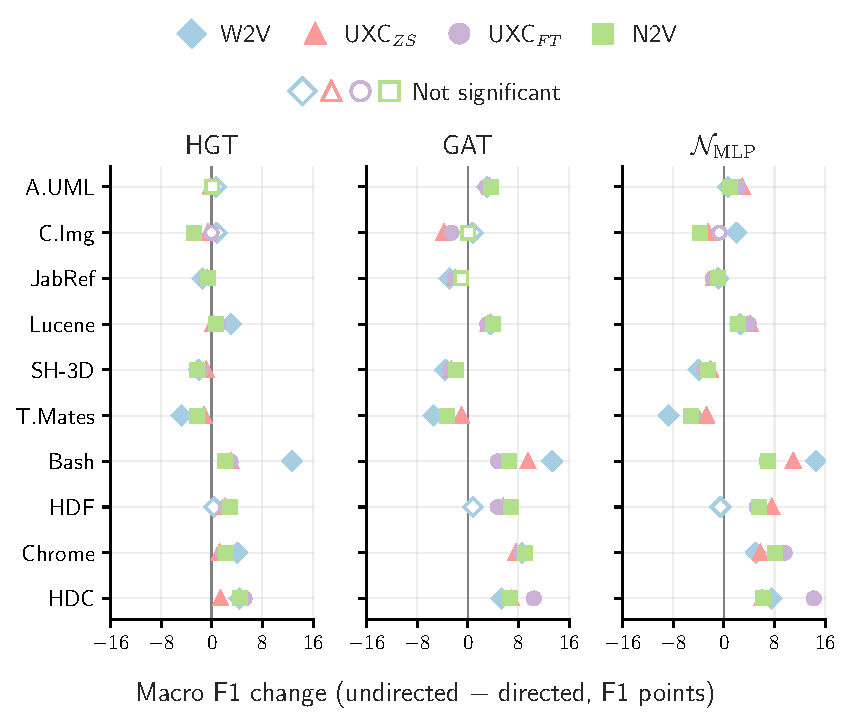
\includegraphics[width=1\columnwidth]{Images/rq3_direction_f1_macro.pdf}
\caption{Change in macro-F1, in F1 points, from directed to undirected aggregation (undirected $-$ directed) for each predictor and input representation; negative values mean directed aggregation scored higher. Each point is the median over 100 paired splits; hollow markers are not significant.\label{fig:rq3_direction}}
\end{figure}

\parg{Which predictor scores highest?} Figure~\ref{fig:rq3_agg} pools the ten systems with undirected neighbors: each point is the median of one system and the boxes show the spread across systems. GAT has the highest median macro-F1 with every representation and the highest median micro-F1 with every representation except Node2Vec, where HGT is marginally higher. GAT also scores highest most often: in each split we count which of the four predictors scores highest, and GAT has the largest share of wins, averaged over systems, with every representation and on both metrics. All three predictors with neighborhood aggregation exceed the MLP without neighbors in every median comparison. As without neighbors, \ft{} has the highest median macro-F1 across systems for every predictor, with GAT and \ft{} giving the highest scores overall.

Most of the variation in F1 lies between systems and not between runs of one system. The choice of predictor matters most for Word2Vec and \zs{}, the two representations without dependency information, and less for Node2Vec and \ft{}.

\begin{figure*}[h]
\centering
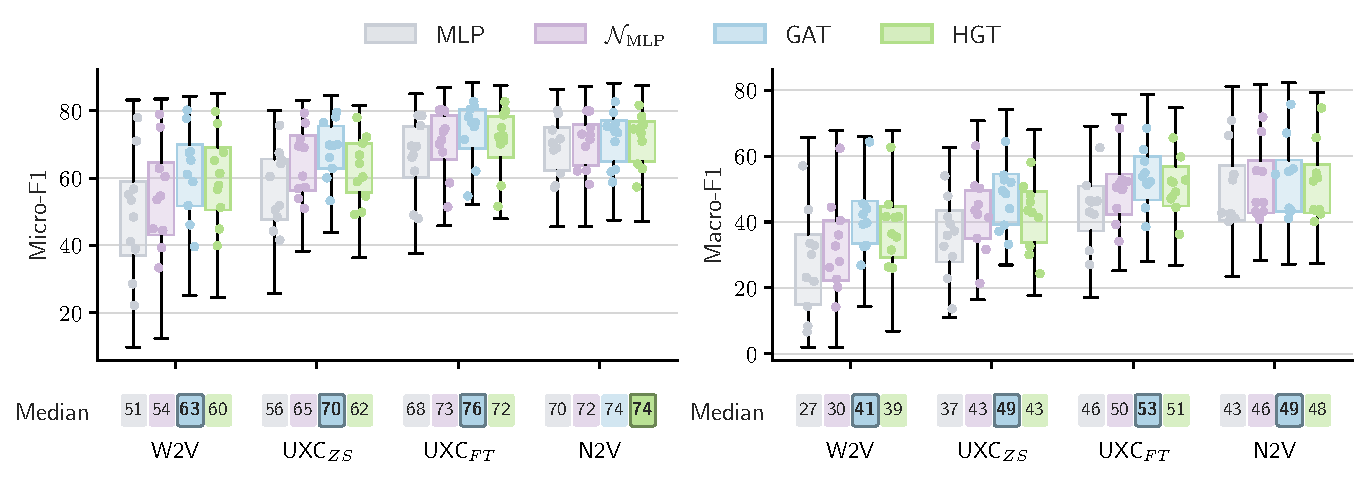
\includegraphics[width=0.98\textwidth]{Images/rq3_fig_compare_undirected.pdf}
\caption{Micro-F1 (left) and macro-F1 (right) of the MLP, \mlp{}, GAT, and HGT with undirected neighbors, by input representation. Each point is the median of one system over 100 runs; boxes show the spread across systems, and the values below are the median of medians across systems, with the highest in each group in bold.\label{fig:rq3_agg}}
\end{figure*}

\begin{GrayBox}{Answer to RQ3.}
Dependency neighbors do not benefit all predictors equally. With undirected aggregation, median changes are positive for every predictor and representation, but GAT and the \mlp{} improve more consistently across systems than HGT, which shows significant losses in some cases. Directed aggregation is less reliable, particularly with Node2Vec, where median macro-F1 decreases for all three predictors. Although undirected aggregation generally gives larger gains, it is not preferable on every system: several systems consistently favor directed aggregation across predictors and representations. These comparisons also change neighborhood size, so they do not isolate direction alone. With undirected neighbors, GAT has the highest median macro-F1 across systems for every representation, and \ft{} remains the strongest representation by this measure for every predictor.
\end{GrayBox}